\chapter{Bilan et Guide d'utilisation du \textit{Clustering Interactif}}
\label{chapter:5-GUIDE}
	
	% Introduction.
	Dans nos études, nous nous sommes intéressés aux assistants conversationnels orientés par tâches et aux méthodes de conception des bases d'apprentissage nécessaires à leur entraînement.
	Dans ce chapitre, nous dressons une synthèse des découvertes et des conseils d'utilisation de notre méthodologie d'annotation basée sur un \texttt{Clustering Interactif} ayant pour but d'assister les experts métiers dans la phase de modélisation des textes en intentions de dialogue.
	
	%%%%%--------------------------------------------------------------------
	%%%%% Section 5.1:
	%%%%%--------------------------------------------------------------------
	\section{Présentation rapide du \textit{Clustering Interactif} et de ses avantages}
		\label{section:5.1-GUIDE-PRESENTATION-RAPIDE}
		
		% Détails de fonctionnement.
		\todo[inline]{
			SECTION À RÉDIGER: \\
			- trouver une base d'apprentissage acceptable, puis corriger manuellement \\
			- intervention d'experts métiers sur la base de leur connaissance métiers \\
			- revues d'annotations basée sur leur connaissance métiers \\
			- aide à la modélisation par le \textit{clustering}
		}
		
		% Constat : expert métier pas à leur place !
		Nous partons du constat selon lequel les tâches de modélisation et d'annotation de textes en intentions sont connues pour être complexes, subjectives et sensibles aux erreurs (voir \textsc{Section~\ref{section:2.3-DEFIS-ANNOTATION}}).
		Ainsi, les experts métiers intervenant au sein d'un projet de conception d'une base d'apprentissage pour un assistant conversationnel 
		%Nous partons du constat selon lequel les experts métiers qui modélisent et annotent les textes en intentions sont généralement mal intégrés au sein d'un projet de conception d'une base d'apprentissage.
		En effet, ces derniers sont confrontés à des problèmes analytiques ou techniques pour lesquels pas des compétences analytiques et techniques tâches sont connues pour être complexes, subjectives et sensibles aux erreurs (voir \textsc{Section~\ref{section:2.3-DEFIS-ANNOTATION}}), demandant des compétences analytiques et techniques 
		
		reposant sur le cycle \texttt{MATTER} (\cite{pustejovsky-stubbs:2012:natural-language-annotation}), 
		De ce fait, les experts métiers intervenant dans le projet 
		% selon lequel les experts métiers, ayant les compétences pour valider la pertinence  sont mal intégrés dans les projets de conception de bases d'apprentissage nécessaires à l'entraînement de modèles supervisés de \textit{Machine Learning}.
		
		% Proposition d'un \texttt{Clustering Interactif}.
		Pour assister cette phase de modélisation, et dans le but de recentrer l'intervention des experts métiers sur leurs compétences (métiers, et non analytique , nous proposons une nouvelle méthode d'annotation basée sur un \texttt{Clustering Interactif}.
		Cette
		
		\begin{leftBarImportantGreen}
			La \textsc{Figure~\ref{figure:5.1-GUIDE-PRESENTATION-RAPIDE-CLUSTERING-INTERACTIF}} ...
			
			% Figure.
			\begin{figure}[H]
				\centering
				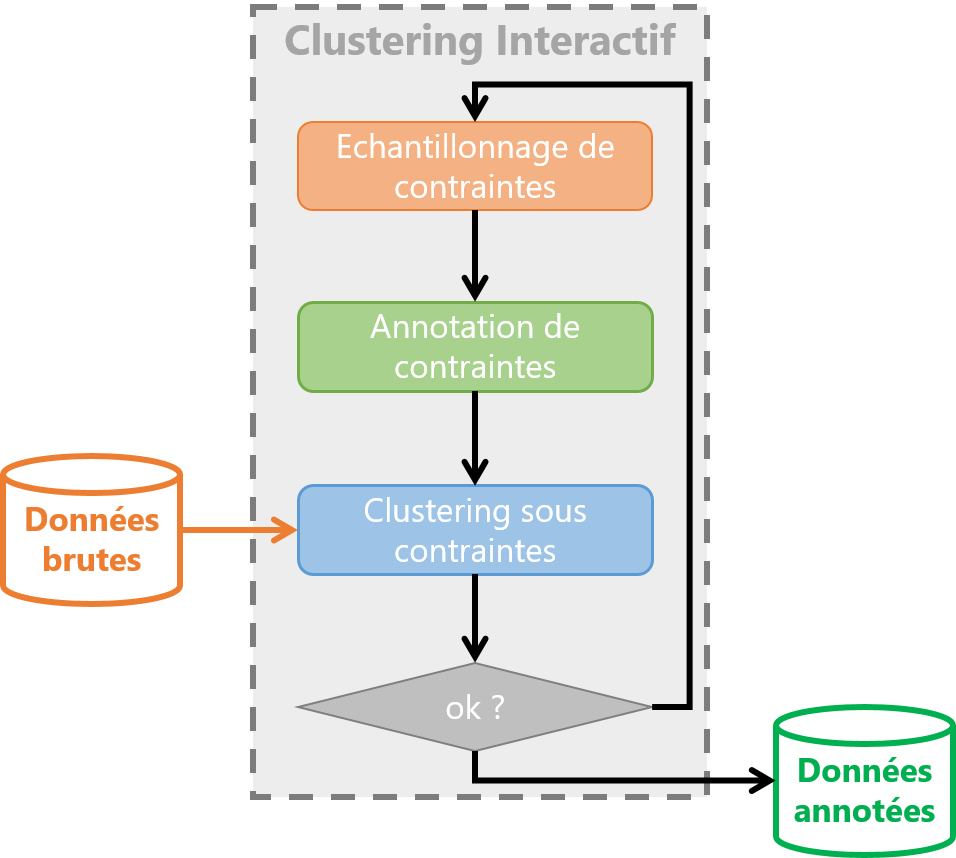
\includegraphics[width=0.95\textwidth]{figures/interactive-clustering-architecture-sequentielle}
				\caption{
					Schéma illustrant l'architecture du \texttt{Clustering Interactif}.
					La boucle principale enchaîne un échantillonnage de couples de données, une annotation de contraintes, et un \textit{clustering} sous contraintes.
				}
				\label{figure:5.1-GUIDE-PRESENTATION-RAPIDE-CLUSTERING-INTERACTIF}
			\end{figure}
		\end{leftBarImportantGreen}
	
	
	%%%%%--------------------------------------------------------------------
	%%%%% Section 5.2:
	%%%%%--------------------------------------------------------------------
	\section{Conseils pour organiser l'annotation}
		\label{section:5.2-GUIDE-ANALYSE}
		\todo[inline]{
			SECTION À RÉDIGER: \\
			- bien définir l'objectif à modéliser (par action ? par objet ?) \\
			- laisser à la mach \\
			- faire référence aux maximes de \cite{leech:1993:corpus-annotation-schemes} ?
			1. VOIR LA DONNEE NON PRETRAITEE: It should always be possible to come back to initial data (example BC). Note: can be hard after normalization ("l'arbre !" vs "le arbre", etc.) \\
			2. ANNOTER DES DIFFERENCES VISIBLES: Annotations should be extractable from the text \\
			3. DOCUMENTER L'AJOUT DE CONTRAINTES: The annotation procedure should be documented (ex: Brown Corpus annotation guide, Penn Tree Bank annotation guide) \\
			4. DOCUMENTER LES COMPETENCES DES ANNOTATEURS: Mention should be made of the annotator(s) and the way annotation was made (manual/automatic annotation, number of annotators, manually corrected/uncorrected...) \\
			5. SUBJECTIVITE => 3 ANNOTATEURS: Annotation is an act of interpretation (cannot be infallible) \\
			6. MIEUX VAUT NE PAS LIER QUE LIER DE MANIERE AMBIGUE: Annotation schemas should be as independent as possible on formalisms \\
			7. PLUSIEURS VISIONS POSSIBLES, IL FAUT EN CHOISIR UNE ET S'Y TENIR: No annotation schema should consider itself a standard (it possibly becomes one)
		}
	
	
	%%%%%--------------------------------------------------------------------
	%%%%% Section 5.3:
	%%%%%--------------------------------------------------------------------
	\section{Conseils pour analyser les résultats}
		\label{section:5.3-GUIDE-ANALYSE}
		\todo[inline]{
			SECTION À RÉDIGER: \\
			- Cas d'arrêt quand le \textit{clustering} stagne à 5\% : si change pas, alors l'annotation n'a plus d'effet... \\
			- utiliser le graphe de contraintes pour voir les données liées entres elles et les données isolées \\
			- Analyse avec résumer par LLM pour identifier facilement les thématiques qui se dégagent \\
			- Analyse avec FMC pour identifier le vocabulaire qui caractérise chaque thématique \\
			- utiliser ces analyses pour régler le nombres d clusters ?
		}
	
	
	%%%%%--------------------------------------------------------------------
	%%%%% Section 5.4:
	%%%%%--------------------------------------------------------------------
	\section{Conseils pour paramétrer la méthode}
		\label{section:5.4-GUIDE-PARAMETRAGE}
		\todo[inline]{
			SECTION À RÉDIGER: \\
			- Architecture parallele : pour gagner du temps\\
			- paramétrage optimal: simple + tfidf + kmeans + closest \\
			- taille de batch d'annotation dépendant de la taille du jeu de données (dépend du temps de clustering)
		}
	
	
	%%%%%--------------------------------------------------------------------
	%%%%% Section 5.5:
	%%%%%--------------------------------------------------------------------
	\section{Estimation des coûts du projet d'annotation}
		\label{section:5.5-GUIDE-COUTS}
		\todo[inline]{
			SECTION À RÉDIGER: \\
			- rappeler les équations de temps: environ 24 x taille de dataset, sans les revues d'annotations \\
			- besoin de 3 annotateurs pour confronter les vision et modéliser dans de bonnes conditions. organiser les revues sur la base des différences entre cas d'usage métier \\
			- ajouter de la redondance si le cas d'usage est complexe, mais ça ralenti \\
			- avantage par rapport aux méthode usuelles : moins abstrait/complexe, moins d'essai-erreur
		}